\documentclass[12pt]{article}

\usepackage{lmodern}	% for nice Fonts
\usepackage{graphicx}	% For adding pictures
\usepackage[font=small,labelfont=bf]{caption}  % Caption formatting
\usepackage{subcaption}

\usepackage{hyperref}


%for editing purposes
\usepackage{color}

\title{Curly-Squeegee Process Book}
\author{ Brian Kimmig \& Jimmy Moore}
\date{\today}


\begin{document}
\maketitle

\begin{abstract}
	Curly-Squeegee (CS) is a web-bsaed tool for visualizing and exploring actor filmographies in an interactive way. By enabling users to search for their favorite actors and see their entire body of work displayed a variety of ways, we hope it invites them to explore the different views, select and filter different sub-sets of actor filmography data, and find intersting or surprising hidden trends.
\end{abstract}

\newpage

\tableofcontents

\newpage


\topskip0pt
\begin{center}

	\vspace*{\fill}
	\textit{To ourselves $\cdots$ for always being there.}
	\vspace*{\fill}
	
\end{center}

\newpage 

\section{Editing notes}

{\color{red}

Depending on how thourough we want to be (and how much time we have for thoroughness) we could incorporate any of the talking points from the ``example" documents
\begin{itemize}
	\item \href{http://dataviscourse.net/2015/assets/process_books/bansal_cao_hou.pdf}{Real time audio visualization project - Soundscapes}
	\item \href{http://dataviscourse.net/2015/assets/process_books/walsh_trevino_bett.pdf}{Oh Shit, earthquakes!}
	\item Compile a bunch of good funny gifs we could use as loading images.  pick from them with a randomizer function.
\end{itemize}

Options include:
\begin{enumerate}
	\item Explicit analysis on color choices, modes of comparison (length, hue, etc)
	\item in-depth explanation of our  choice of design principles or encodings \textbackslash visual variables
	\item Analysis of data
	\item place a \textbf{'Loading...'} message on loading screen.
\end{enumerate}
}

\newpage

\section{Project Background}

\subsection{Motivation}\label{sec:Motivation}
	The idea for this project came from the fact that both developers watch a good amount of movies and enjoyed sites like IMDB and RottenTomatoes, but wanted something that focused on specific actors rather than being movie-centric. CS is their solution to needing to sift through lists and text to appreciate a given actors filmography. In three views, one can see their entire body of work as a timeline, with length and color encodings for film-output and film-quality, respectively, as well as career visualizations showing the breakdown of movie genre over the course of their career and a multi-axis interactive plot to explore an actors output as a function of date ranges, ratings, box office earnings, and directors.
	
	CS is meant to provide a new way of viewing actor data, and seeks to facilitiate a fun and interactive web-based solution to questions like:


	\begin{itemize}
		\item How many movies has an actor acted in?
		\item Has an actor been type-cast to a specific genre?
		\item What is the best movie they have made? The worst?
		\item Do they consistently star in well-reviewed films?
		\item Has their career had a golden period in which they were particularly busy, or appeared in well-reviewed films?
	\end{itemize}
	
\subsection{Intended Audience}
Curlee Squeege is geared towards the general public and offers something of interest to the casual movie-goer  and film buff, alike.  

The interface is clean and self-explanatory.  
Users are presented with a short text prompt describing the purpose of the site, a text query box, and a list of trending actors.This presentation allows them to start using the tool immediately with little explanation.

We hope that the site design and visualization aesthetics make it a natural and easy tool to use.
\newpage 

\section{Data Collection}
	In order to build the database needed to visualize an actor's work, we explored several film-related API's.  After some searching, we found the majority were poorly populated, did not have the data we wanted, or charged for use.  We were able to identify two options which allowed us to proceed: \href{http://api.myapifilms.com/index.do}{My API Films} and \href{http://www.omdbapi.com/}{Open Movie Database}. We have set up a web framework using node.hs and Meteor which uses a RESTful architecture to gather API calls via GET requests. We store all data in a MongoDB database. This dataset is fairly dynamic since we rely on user queries to pull the necessary information from the APIs.

	
	\begin{center}
	\color{blue}
	\textbf{Do we want to have a breakdown or description of the API call, data retrieval, and database storage? }
	\end{center}
	
\subsection{Data Processing}
	API requests are returned in JSON format, so there is little clean-up beyond. Returned data is fairly detailed, so we selectively cull certain uncessary fields and aggregate filmography data based on what we want to visualize. We have two data structures in our databases:
	
	\begin{itemize}
		\item Actor Table: This stores all the actor information of a selected actor, including the movies they've acted in.
		\item Movie Table: This contains all of the information for each movie we wish to plot or visualize.
	\end{itemize}

	The data collection and filtering is probably the most sophisticated portion of this project. With everything stored and readily accessible, we use built-in javascript math functions and agregate parameter counts of our actor data to illustrate actor filmographies.

\subsection{Data Formatting}

talk about filter and utils functions?
\subsubsection{Only Visualizing Films}
	
	\begin{itemize}
			\item Mention Tom waits case where his most popular work was soundtracks
			\item Talk about formatting for films which are currently released (and therefore have data/votes).
	\end{itemize}
	
\subsubsection{Formatting numbers}
	
	\begin{itemize}
		\item Remove NA from votes
		\item removing commas from votes
		\item formatting years
	\end{itemize}


\newpage 

\section{Project Interface}

Thanks to our accelerated development schedule, we were able to move from sketch book to implementation very quickly. We brainstormed multiple views for this project with the goals of answering the questions raised in section \ref{sec:Motivation} for a variety of actors, as well as encouraging user exploration and re-use.  

In the interest of time, we ultimately decided on four views:  Two main visualizations ( Actor Filmography and a Parallel Axis Chart)and two more easily implemented graphics -- an aggregte genre view, and tree map of common co-stars.

The following subsections discuss how we approached implementing and styling each interface, and how\textbackslash why it evolved during the life of the project.  

\subsection{Landing Page}

Our original design goals always envisioned this as an interactive web-based tool.  We did not want to rely on a static dataset, and instead wanted to tap into the large datasets of cinema history to create actor filmographies, applicable to any actor, from any time. for the most flexible and fun experience.   Taking a cue from Google's clean and austere design, we wanted a plain front page with minimal clutter.  
	\begin{figure}[h!]
		\centering
		\begin{subfigure}[t]{.5\textwidth}
			  \centering
			  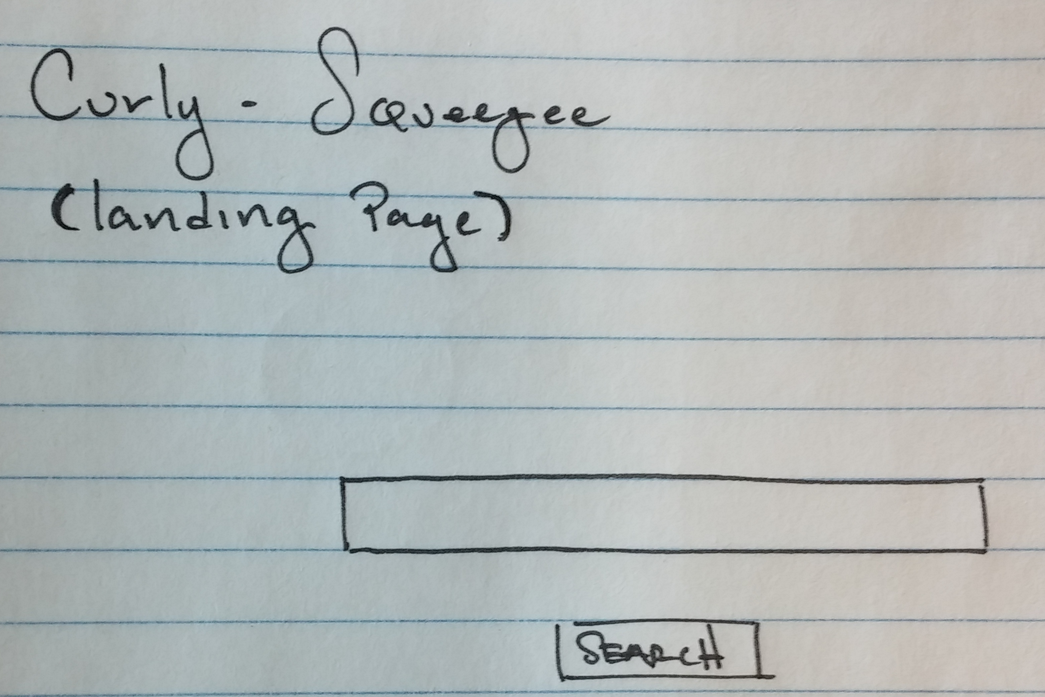
\includegraphics[width=\linewidth]{images/landingPage_crop.png}
			  \caption{Original design sketch}
			  \label{fig:sub1}
		\end{subfigure}%
		\begin{subfigure}[t]{.8\textwidth}
			  \centering
			  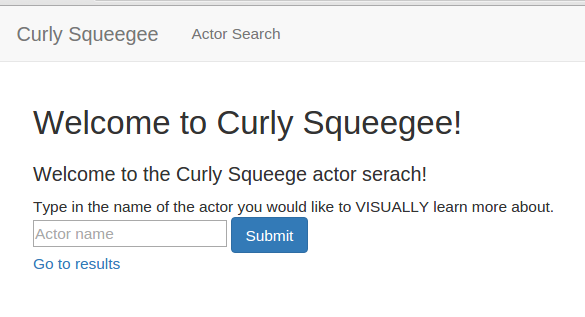
\includegraphics[width=0.75\linewidth]{images/landingPage.png}
			  \caption{Current implementation}
			  \label{fig:sub2}
		\end{subfigure}%
		\caption{Landing page development}
		\label{fig:landingPage}
	\end{figure}

In implementing this design we added some explanatory text, as well as a list of trending actors which can serve as a starting point for new users.  After reading the site description, the user has the choice to click any one of the provided actors, or input one of their own.

\subsection{Loading Page}

Once the user has made their selection, the node.js framework takes that search query and polls the MyAPIFilms and OMDB API's to collect the necessary actor information.  Fulilling these requests can take some time, so we display a loading gif to indicate that the process is ongoing.

			\begin{figure}[h!]
				\centering
				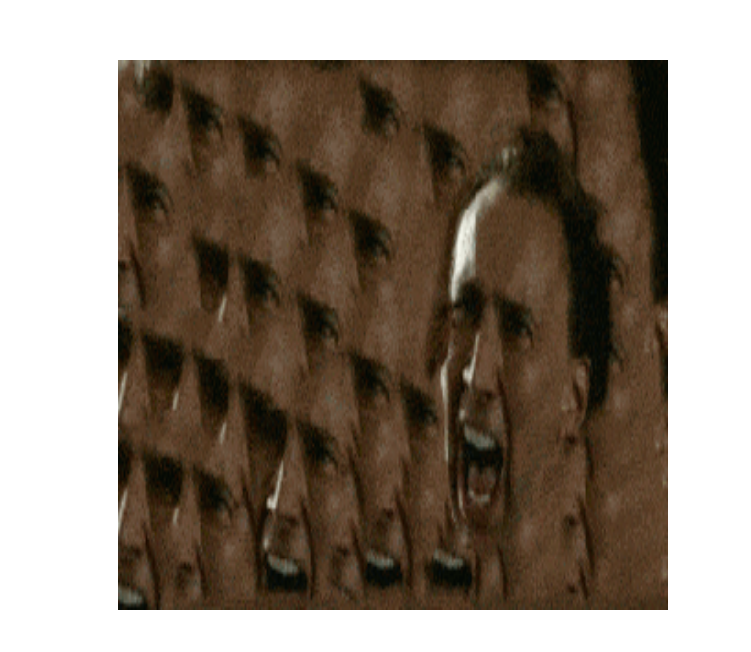
\includegraphics[scale=0.3]{images/loadingPage.png}
				\caption{After the user submits a search query, the application waits for the API calls to complete and fetch the actor's filmography. An animated gif can help pass the time.}
			\end{figure}

Wait times to complete a search request depend on the actor's catalog of work and also on the speed of the user's internet connection.  We ave experienced pauses of 30 seconds to 5 minutes, though typical queiries return within 2 minutes.

\newpage 

\section{Visualizations}
Once all API calls have completed and the data is saved in our database, we load the `results' page, which is where each visualization is displayed.  The  filmography has been loaded, we load our results page', showcasing our multiple views and actor information.

\subsection{Actor Fact Box -- Depricated}

\textbf{Note:}  This section was removed from the final release. We decided it did not contribute to the overall presentation and was at odds with the interface style we were hoping to create.  The text remains for  historical analysis.


\textit{ (Depreicated)	This data serves as an orientation tool,indicating to the user whether the correct actor was returned.  This is particularly important in cases when searching for actors with common names.  Using the OMDB API data, we are able to display a photograph of the actor, their full name, date of birth, and other derived data from the API call.  We currently display their total number of films.  other useful information would be when they started acting \textbackslash first credited role, years active, and highest or worst rated movie.}
	
		\begin{figure}[h!]
			\centering
			\begin{subfigure}[t]{.5\textwidth}
				  \centering
				  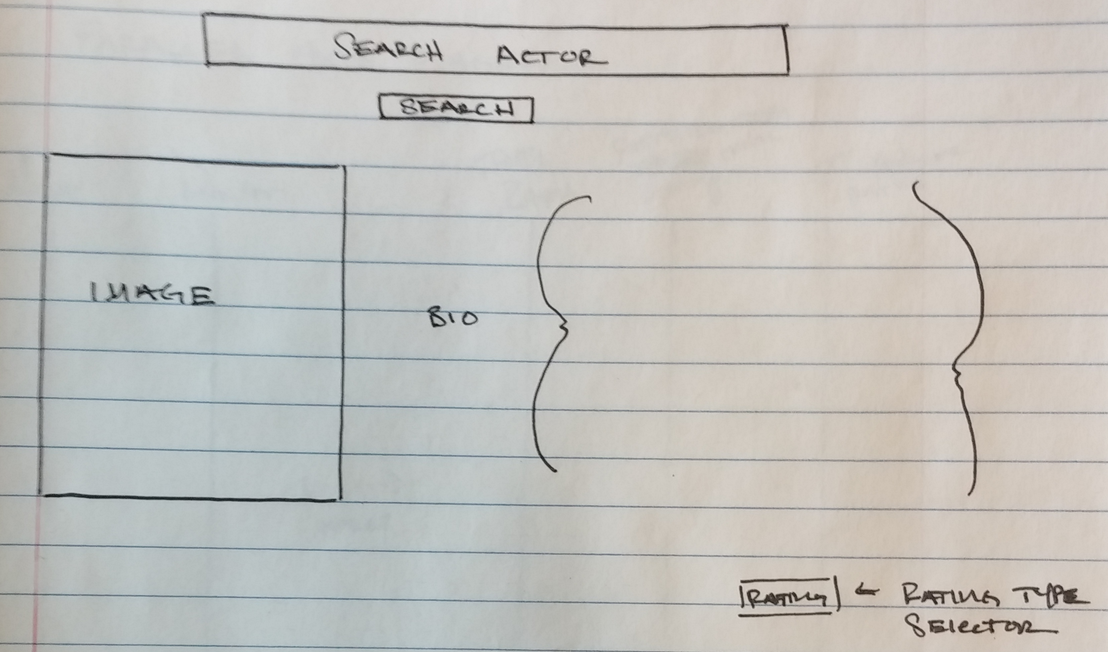
\includegraphics[width=\linewidth]{images/actorFactBox_crop.png}
				  \caption{Original design sketch}
				  \label{fig:sub1}
			\end{subfigure}%
			\begin{subfigure}[t]{.5\textwidth}
				  \centering
				  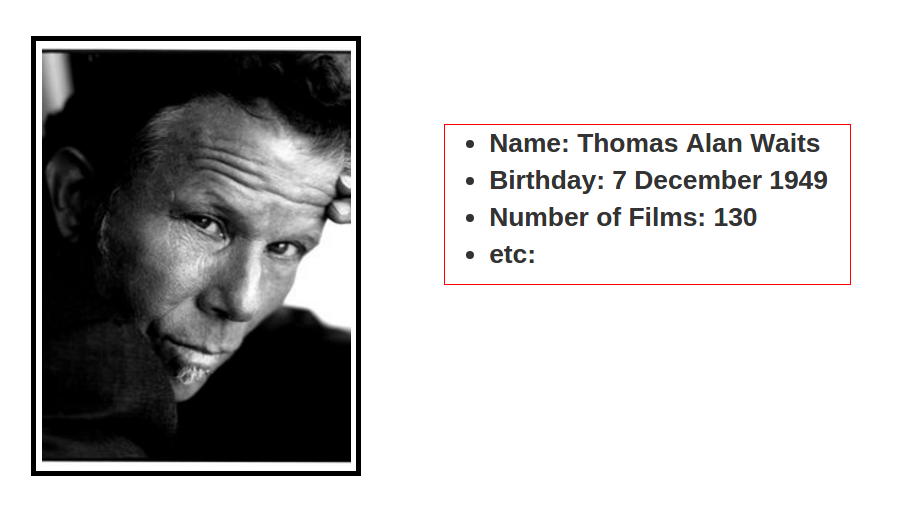
\includegraphics[width=.8\linewidth]{images/actorBox.png}
				  \caption{Current implementation}
				  \label{fig:sub2}
			\end{subfigure}%
			\caption{Actor `Fact Box' development}
			\label{fig:actorFactBox}
		\end{figure}


\subsection{Filmography Timeline}

	\begin{figure}[h!]
			\centering
			\begin{subfigure}[t]{.5\textwidth}
			  \centering
			  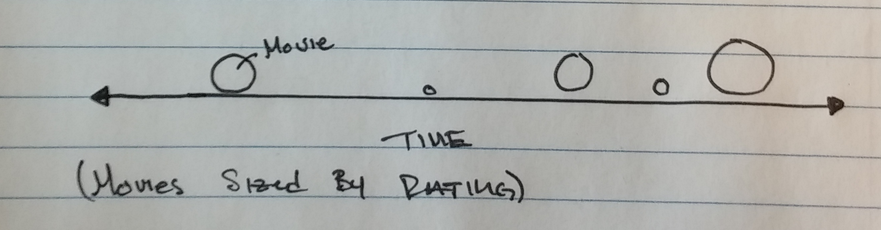
\includegraphics[width=\linewidth]{images/timeline_orig.png}
			  \caption{Original design sketch}
			  \label{fig:timelineA}
			\end{subfigure}%
			\begin{subfigure}[t]{.5\textwidth}
			  \centering
			  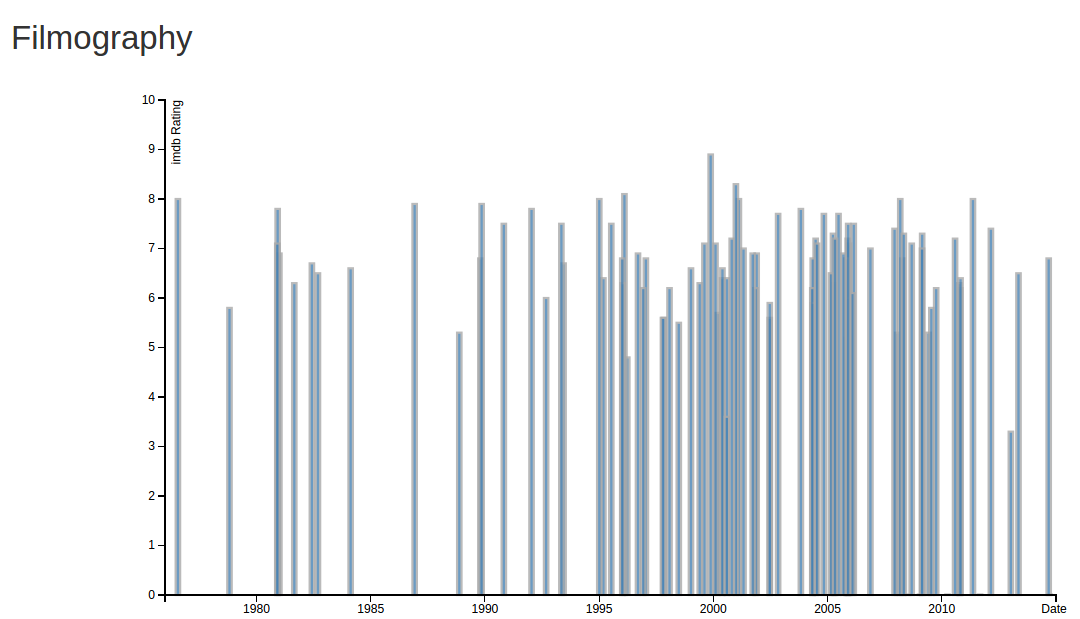
\includegraphics[width=.7\linewidth]{images/timeline_crop_waits.png}
			  \caption{First Implementation}
			  \label{fig:timelineB}
			\end{subfigure}%
			\caption{Timeline development}
			\label{fig:timeline}
		\end{figure}
		
Early in our design phase, we considered using circles on a timeline as a suitable encoding for showing film distribution.  This decision was inspired by the \href{http://mariandoerk.de/edgemaps/demo/#phils;time;;;}{philosophers, poets, and musicians} timeline comparison shown in class. The idea was to visually show the distribution (and density) of an artist's career chronologically and encode information such as film ratings or earnings as the circle radius or fill color.   This decision was later refined after our brainstorming session (Section \ref{sec:Projcet Feedback}). Concerns were raised that actors with frequent and\textbackslash or successful work would create a cluttered timeline visual.  We also recalled thelack of effectiveness with comparing quantitative values when encoded as an area, and decided it would be better to switch to a barchart visual.  This way we could cleanly show movie release dates and have a more direct comparison of ratings or other quantitative data by mapping it to bar height.

As we implemented our barchart visualization, we observed several issues relating to bar sizing, spacing, and overlap.  Consider the filmography of Tom Waits, shown in figure \ref{fig:timelineB}. We did not initially consider visualizing filmographies in the extreme cases of long acting careers, high film output, or areas of dense activity.  In each case, the sizing and spacing of the bars becomes an issue for readability and visual appeal.  Particularly frustrating, were areas where an actor would have multiple films released within a small time frame.  We tried separating these views by using thinner rectangles, adding stroke width to the bars, or introducing opacity.  We were not happy with any of these solutions and sought a better visualization method.

\begin{figure}
	\centering
	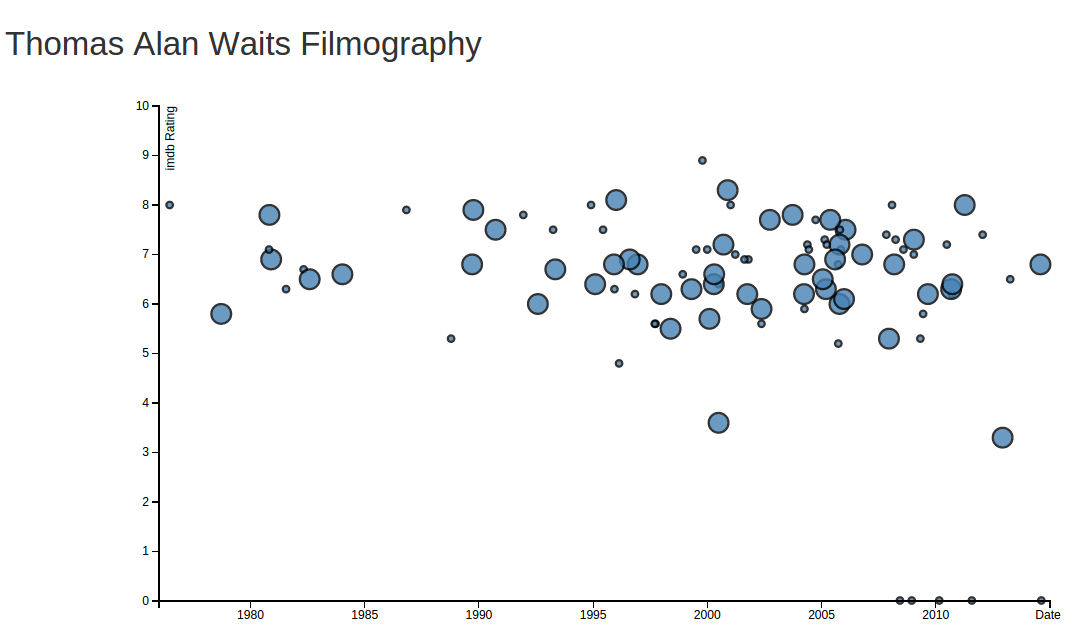
\includegraphics[width=.7\linewidth]{images/timelineC_crop_waits.png}
				  \caption{XY Plot of Tom Waits filmography.  circles are sized by number of  IMDB votes.}
\end{figure}\label{fig:xy}


Figure \ref{fig:xy} is a marked improvement over the earlier efforts to illustrate an actor's filmography.  The XY plot naturally lends itself to an ordered ranking  in each dimension, and the user can immediately identify such information as : high and low ranked films, popular films, and any trend in the actor's career over time.  For example, figure \ref{fig:deniro} verifies the slight decline of  Robert DeNiro's film quality.

\begin{figure}
	\centering
	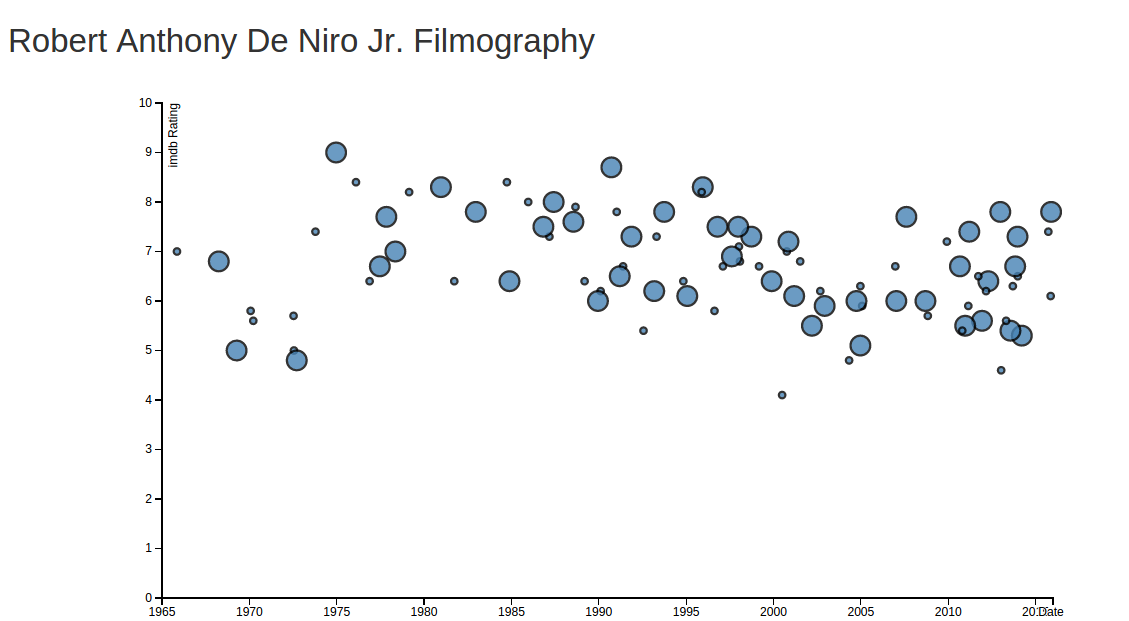
\includegraphics[width=.7\linewidth]{images/Deniro_timeline.png}
				  \caption{We've seen better times.}
\end{figure}\label{fig:deniro}


\subsection{Genre Visualization}

	\begin{figure}[h!]
		\centering
		\begin{subfigure}[t]{.5\textwidth}
		  \centering
		  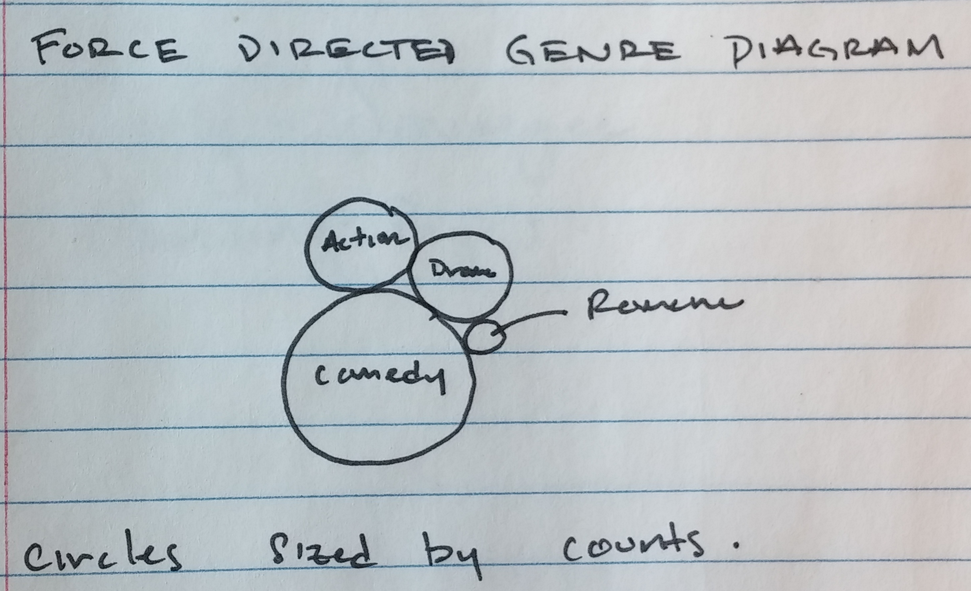
\includegraphics[width=\linewidth]{images/genreVis_crop.png}
		  \caption{Original design sketch}
		  \label{fig:sub1}
		\end{subfigure}%
		\begin{subfigure}[t]{.8\textwidth}
		  \centering
		  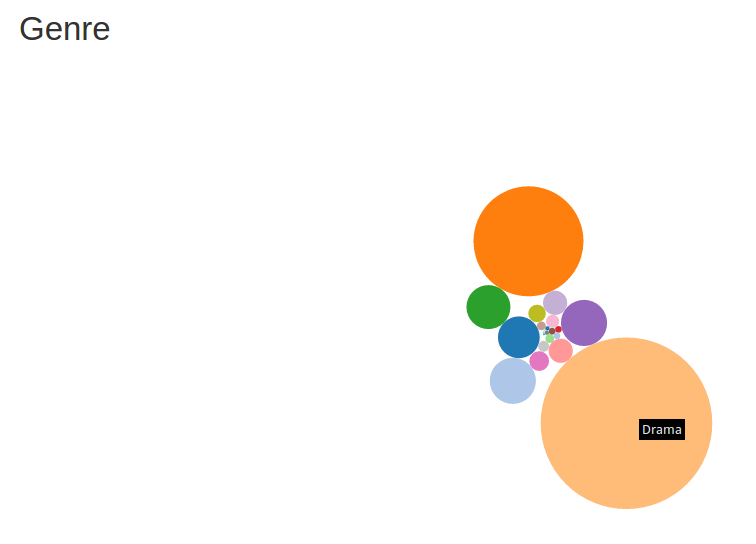
\includegraphics[width=.7\linewidth]{images/genreVis.png}
		  \caption{Current implementation}
		  \label{fig:sub2}
		\end{subfigure}%
		\caption{Genre visualization development}
		\label{fig:genreVis}
	\end{figure}

	
The GenreVis view was an attempt to answer the question of whether an actor gets typecast, or to visualize the proportion of film genres they appear in.  

Each circle represents a unique film genre (Drama, family, comedy, etc.) which is viewable via mouse-hover text.  Th

\subsection{Treemap Visualization of co-workers}


The treemap visualization was a last-minute addition to our project.  We did not orginally plan for such a view, but after the ``Visualizing Maps and Trees'' lecture, we saw a way to group co-stars which have appeared in multiple films alongside the queried actor.

	\begin{figure}[h!]
		\centering
		\begin{subfigure}[t]{.5\textwidth}
		  \centering
		  %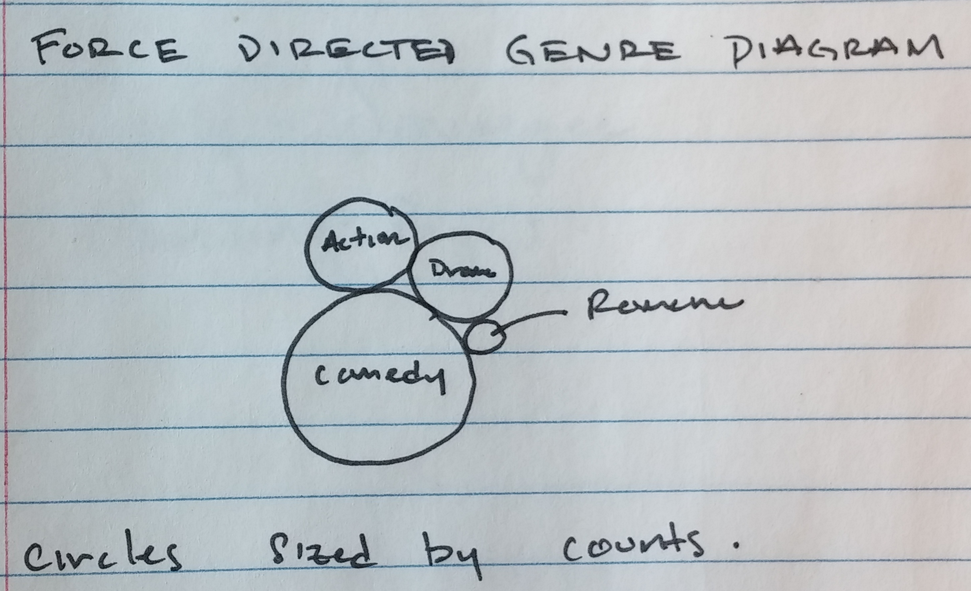
\includegraphics[width=\linewidth]{images/genreVis_crop.png}
		  \caption{Original Implementation}
		  \label{fig:treemapA}
		\end{subfigure}%
		\begin{subfigure}[t]{.8\textwidth}
		  \centering
		  %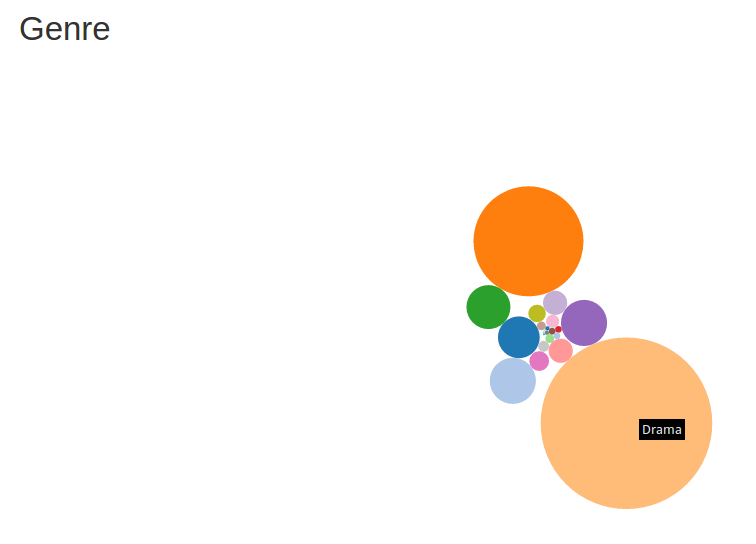
\includegraphics[width=.7\linewidth]{images/genreVis.png}
		  \caption{Current implementation}
		  \label{fig:treemapB}
		\end{subfigure}%
		\caption{Genre visualization development}
		\label{fig:Treemap}
	\end{figure}
	
This view was accomplished in a similar way to the GenreVis view.....	

\subsection{Parallel Axis Coordinate Visualization}
	
From the start, the parallel axis coordinate view was what we were most interested in implementing for this dataset.  We looked forward to determining the highest grossing Schwarzennegar movie from the 80's, or.... \textbf{More}


	\begin{figure}[h!]
		\centering
		\begin{subfigure}[t]{.5\textwidth}
			  \centering
			  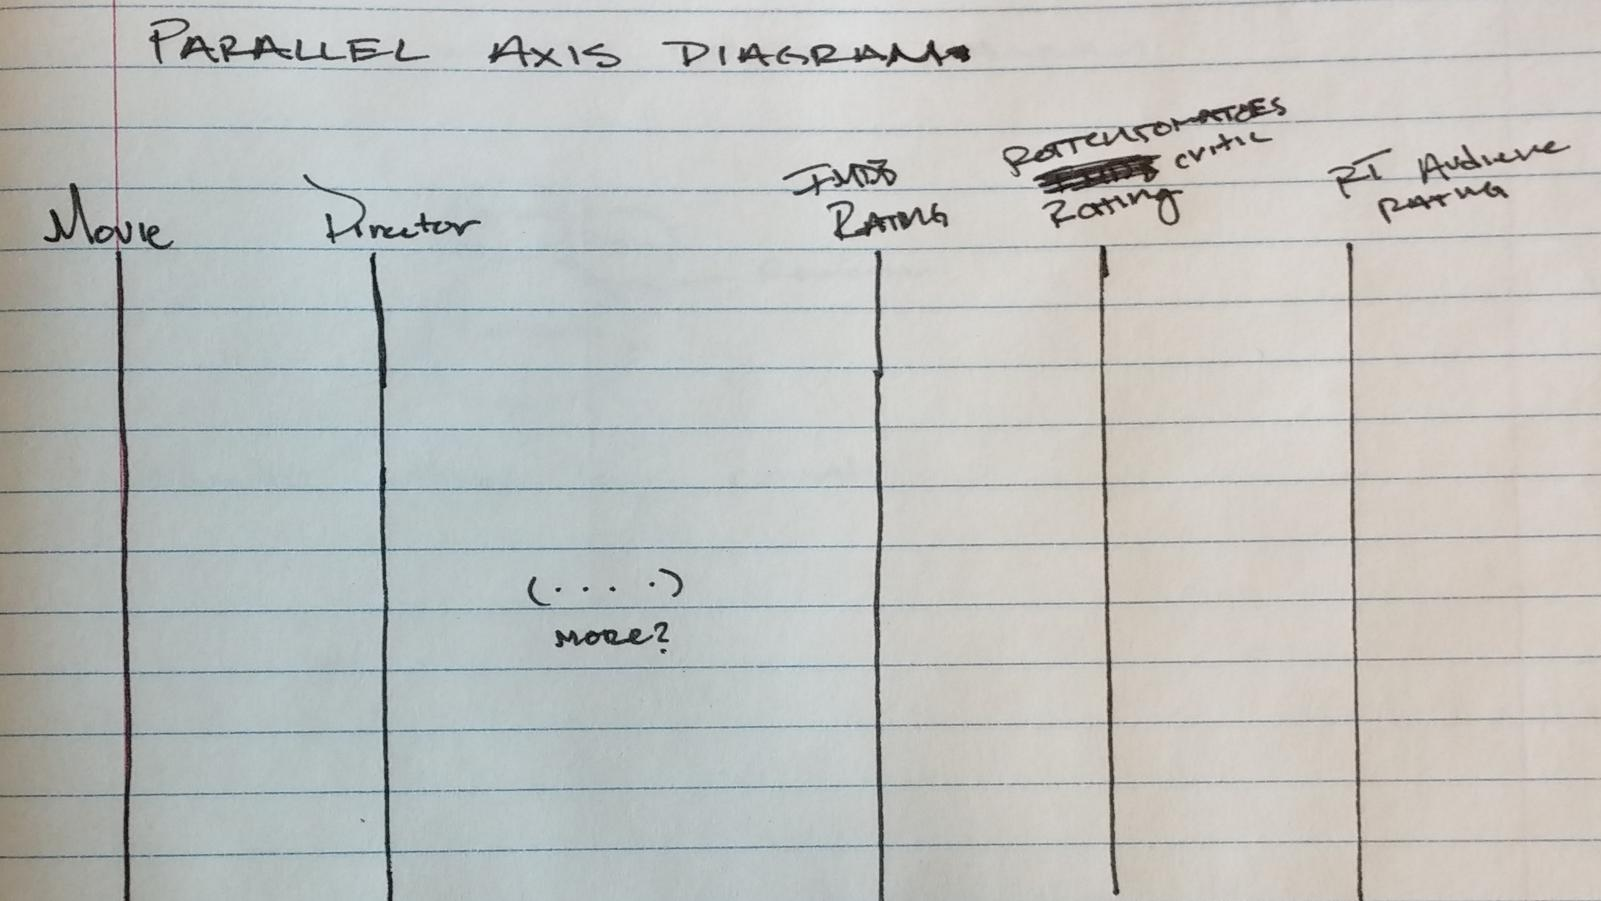
\includegraphics[width=\linewidth]{images/parallel_crop.jpg}
			  \caption{Original design sketch}
			  \label{fig:sub1}
		\end{subfigure}%
		\begin{subfigure}[t]{.8\textwidth}
			  \centering
			  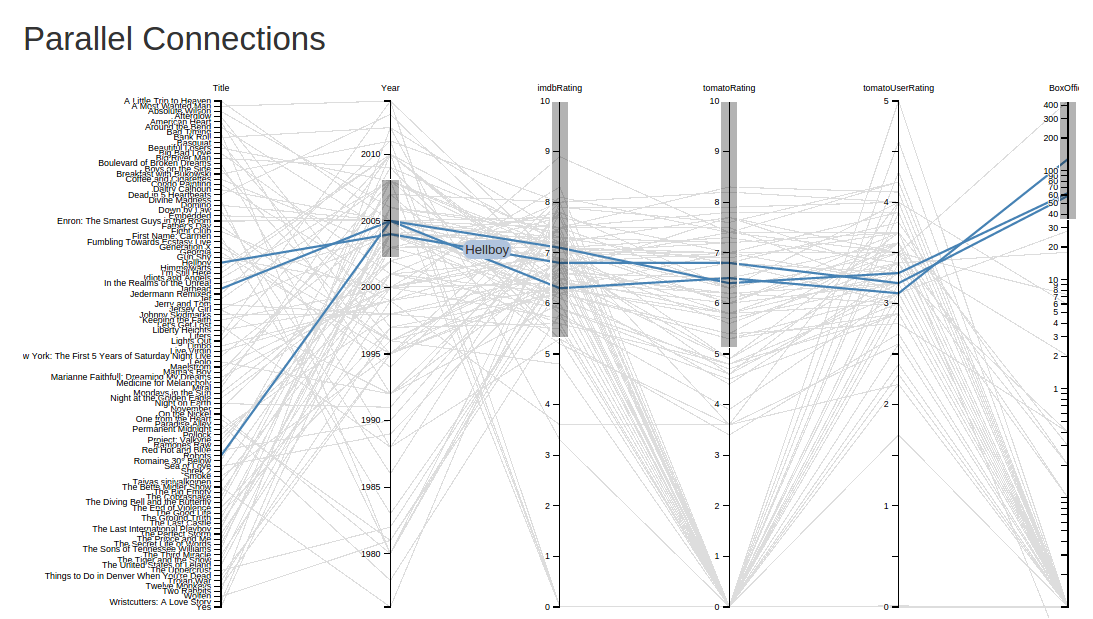
\includegraphics[width=.7\linewidth]{images/parallelAxisCoordVis.png}
			  \caption{Current implementation}
			  \label{fig:sub2}
		\end{subfigure}%
		\caption{Parallel Axis Coordinate visualization development}
		\label{fig:parallelAxisCoordVis}
	\end{figure}



\section{Site Redesign}

Once the views were working and the settings more or less finalized, we decided to work on changing the look of the site.  We wanted to keep the same simplistic look, but benefit from some additional polishing from some pre-packaged CSS and JS styling elements.   

	\begin{figure}[h!]
		\centering
		\begin{subfigure}[t]{.5\textwidth}
			  \centering
			  %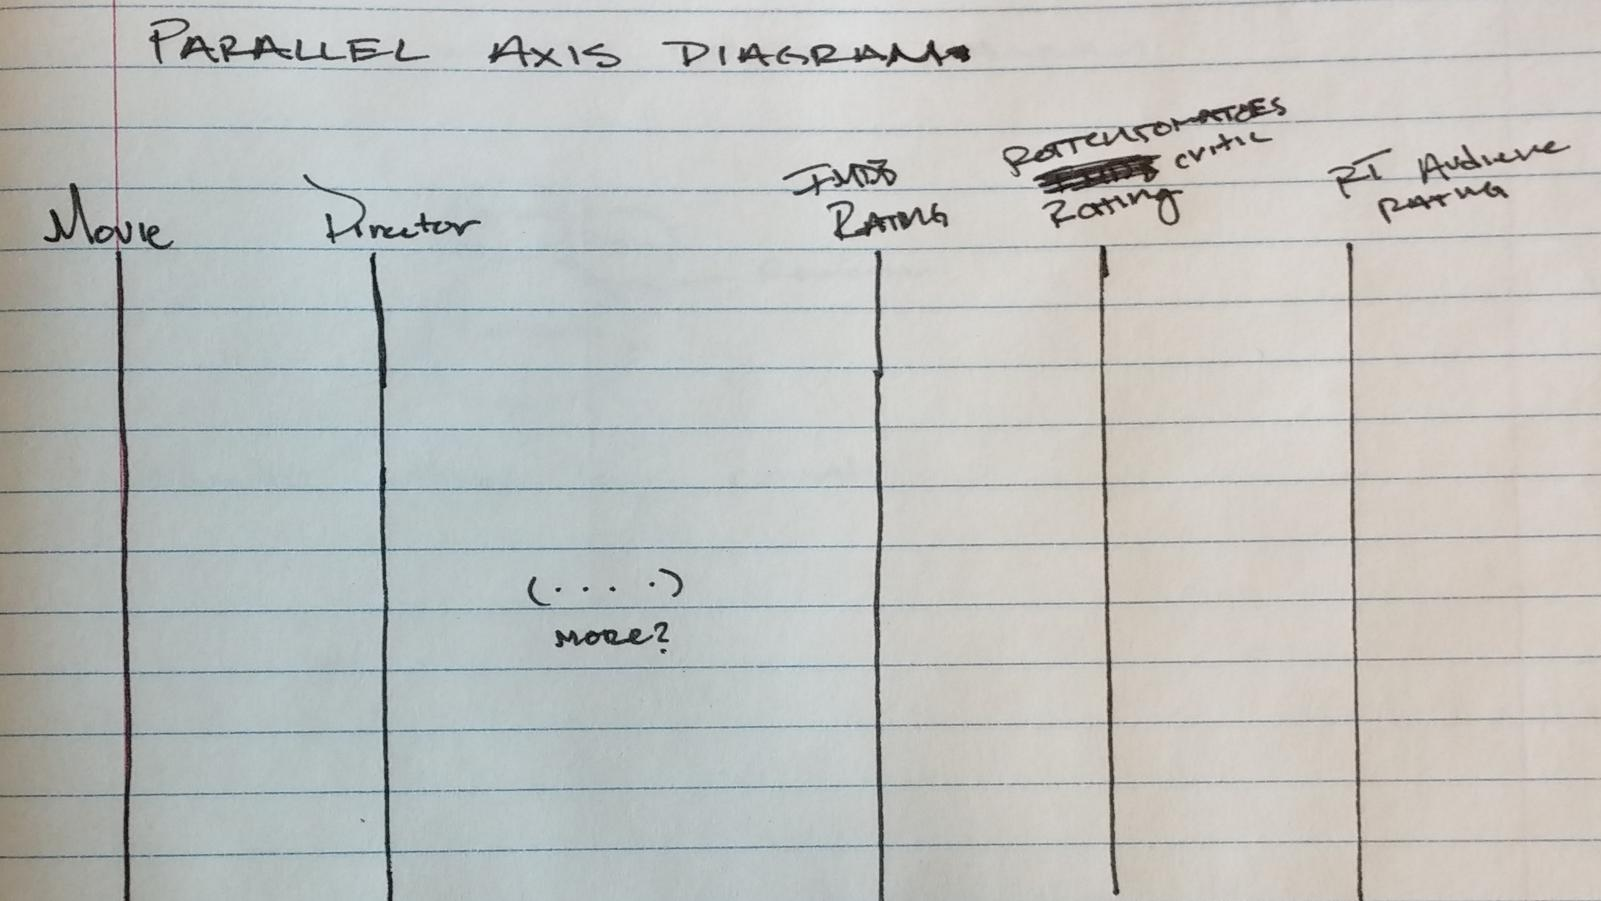
\includegraphics[width=\linewidth]{images/parallel_crop.jpg}
			  \caption{Main Landing Page}
			  \label{fig:redesignA}
		\end{subfigure}%
		\begin{subfigure}[t]{.8\textwidth}
			  \centering
			  %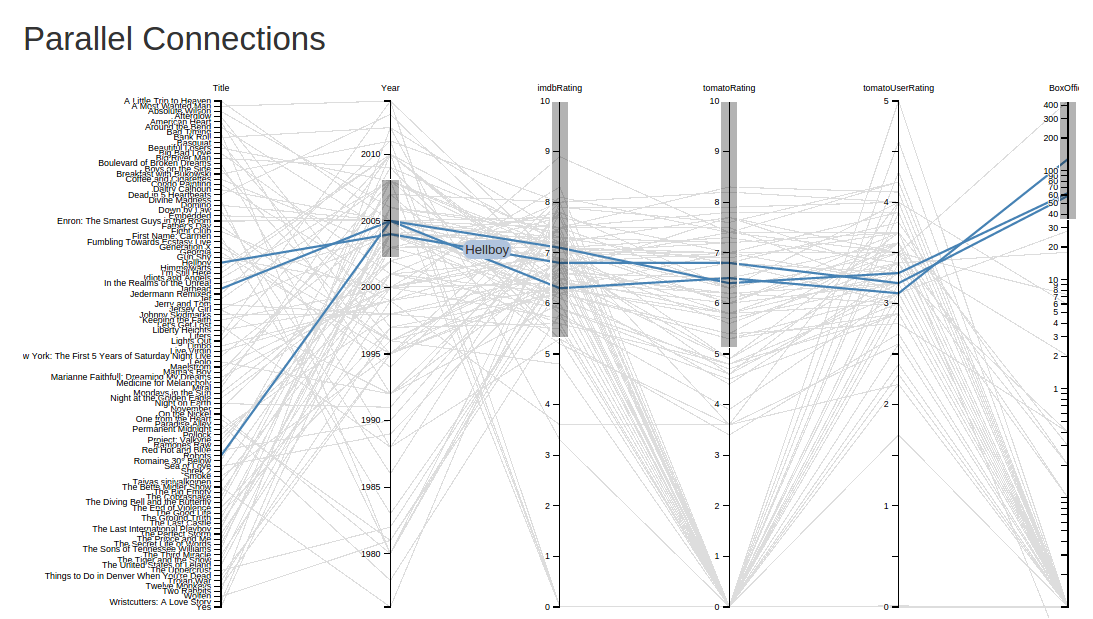
\includegraphics[width=.7\linewidth]{images/parallelAxisCoordVis.png}
			  \caption{Data page}
			  \label{fig:redesignB}
		\end{subfigure}%
		\caption{Site redesign}
		\label{fig:SiteRedesign}
	\end{figure}
We chose the \textbf{XXXXX} located \href{www.google.com}{here} for it's stripped-down appearance, and then \textbf{This JS stuff} for the smooth strolling site-linking functionality.  Since all of our content is essentially on on page, we wanted a clean way to transition between views.

\section{Connected Views}

We chose to interconnect the timelineVis and parallel axis coordinates visualizations so any selected movies in one view would be highlighted in another.  This is especially useful when brushing multiple items in the parallel axis coordinate view and seeing the highlighted distribution of films in the timeline graphic.

This is most useful when visualizing the temporal distrobution of films brushed from the parallel axis plot.  We thought this functionality would help uncover any time trends with given film earnings, directors, etc.

The results of these searches are dependent on the actors, of course.

\newpage

\section{Project Feedback} \label{sec:Projcet Feedback}

After we settled on our design and project implementation, we had the opportunity to present a ``sales pitch"  for Curly-Squeegee to another project team to get their feedback.  We met with Phil Cutler, Ariel Herbert-Voss, and Ian Sohl of the "Legion Profiling Visualization" team. They provided the following feedback:

\begin{itemize}
	\item \textbf{Phil Cutler} (u0764757@utah.edu)
	
	Provided good feedback and constructive criticism. Raised concerns about Parallel axis plot readability in the limit of a long, active acting career as well as a lack of information on new actors. Liked the idea of the filmography visualization, but recommended using bar charts as opposed to circles anchored to a timeline. He thought it was a neat idea, but did not see it's utility. He admitted he does not like watching movies.
	
	
	\item \textbf{Ariel Herbert-Voss} (u0591949@utah.edu)
	
	Overall very positive and excited reaction. she loved the parallel axis plot idea and also agreed with Phil that a bar chart for the filmography timeline would be more effective. She suggested scaling bars either by film rating or number of films in a given period (for a drill-down style barchart), as well as shading a given bar to convey additional information. Ariel is a film buff and saw a great deal of utility in this visualization
	
	\item \textbf{Ian Sohl} (u0445696@utah.edu)
		No additional feedback beyond what Phil and Ariel had to suggest.
\end{itemize}

\newpage

\section{Team Evaluation}

\textit{Brian Kimmig}: Brian was responsible for the API calls, data collection, and database wrangling. His experience as a web developer was very helpful for making this portion of the project proceed smoothly. Brian also created  the genreVis, treep map, and parallel coordinate view.

\textit{Jimmy Moore}: Jimmy contributed code for the Database storage of API calls, and the Actor filmography visualization, along with site design and formatting.  He also was the project scribe and responsible for project documentation.

\newpage

\section{Future Work}


Awesome project and we want to keep working.  Lots of stuff we could do

\begin{itemize}
	\item Add selection/links/buttons to change search query from filmography to director/producer, soundtrack, or other creative capacity.  Additionally, these multiple datapoints could be overlaid on the same graph and separated with color.
	\item Search for multiple actors and compare their filmographies on the timeline visualization.
	\item Create a set view to show which movies any $n$ actors have acted in.  Or show a network visualization of the separation of a number of actors.  Use the individual movies as the graph nodes.  Force directed visualization might be best.
\end{itemize}

\end{document}